\renewcommand{\theequation}{\theenumi}
\begin{enumerate}[label=\arabic*.,ref=\thesubsection.\theenumi]
\numberwithin{equation}{enumi}

\item here
\begin{align}
\vec{d1} = \vec{R} - \vec{P} = \myvec{0\\4}
\\
\vec{d2} = \vec{S} - \vec{Q} = \myvec{-4\\0}
\\
\vec {SP} = \vec P - \vec S =  \myvec{2\\2}
\\
\vec {PQ} = \vec Q - \vec P = \myvec{2\\2}
\\
abs\norm{ \mathbf{\vec{d1}} \times \mathbf{\vec{d2}}} = 
abs\norm{ \mathbf{\myvec{5\\1}} \times \mathbf{\myvec{1\\5}}} = 16
\\
abs\norm{ \mathbf{\vec{SP}} \times \mathbf{\vec{PQ}}} =  abs\norm{ \mathbf{\myvec{2\\2}} \times \mathbf{\myvec{2\\2}}} = 8
\\
\frac{1}{2}abs\norm{ \mathbf{\vec{d1}} \times \mathbf\vec {d2}} = abs\norm{ \mathbf{\vec{SP}} \times \mathbf\vec {PQ}} = 8
\end{align}
from above we can say that tha area of the quadrileteral is equal to the half of the multiplication of its diogonals.thus this is a rhombus.

\begin{figure}[!ht]
	\centering
	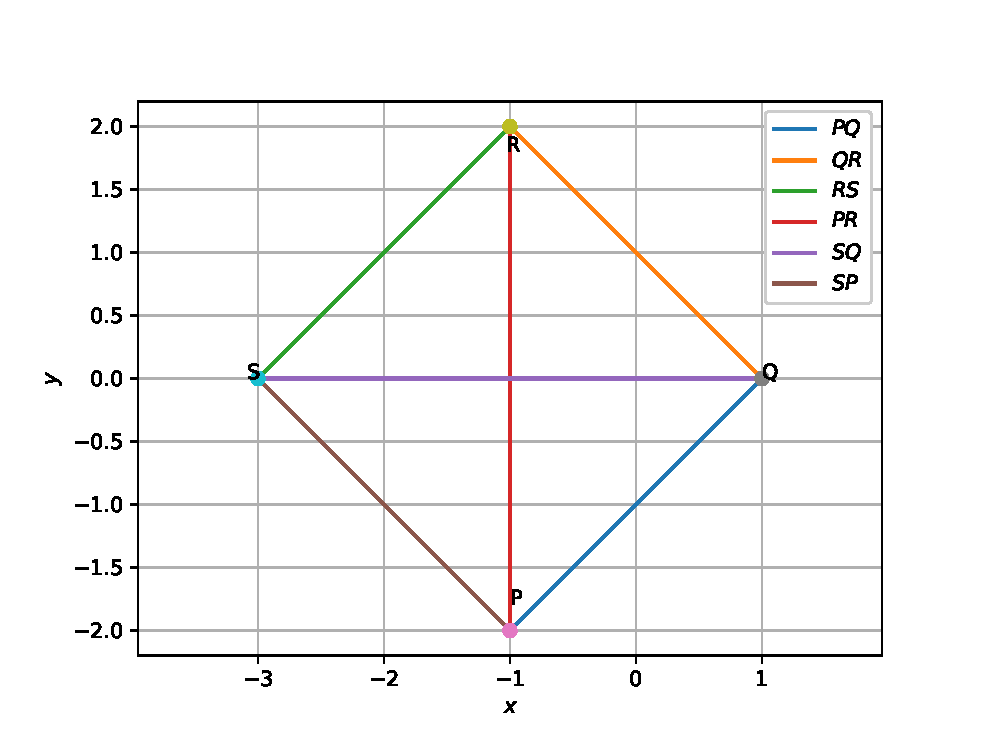
\includegraphics[width=\columnwidth]{./figures/quad1.eps}
	\caption{quadrilateral1 }
	\label{fig:quadrilateral1}
\end{figure}
\begin{lstlisting}
codes/quad1.py
\end{lstlisting}

\item 
\begin{align}
\vec{PQ} = \vec{Q} - \vec{P} = \myvec{6\\-4}
\\
\vec{PR} = \vec{R} - \vec{P} = \myvec{3\\-2}
\\
\vec{RQ} = \vec{Q} - \vec{R} = \myvec{3\\-2}
\\
\vec{PQ} = \vec{PR} + \vec{RQ} = \myvec{6\\-4}
\end{align}
so from above we can say that $\vec P,\vec Q$ and $\vec R$ are linear so it can not be a quadrilateral.

\begin{figure}[!ht]
	\centering
	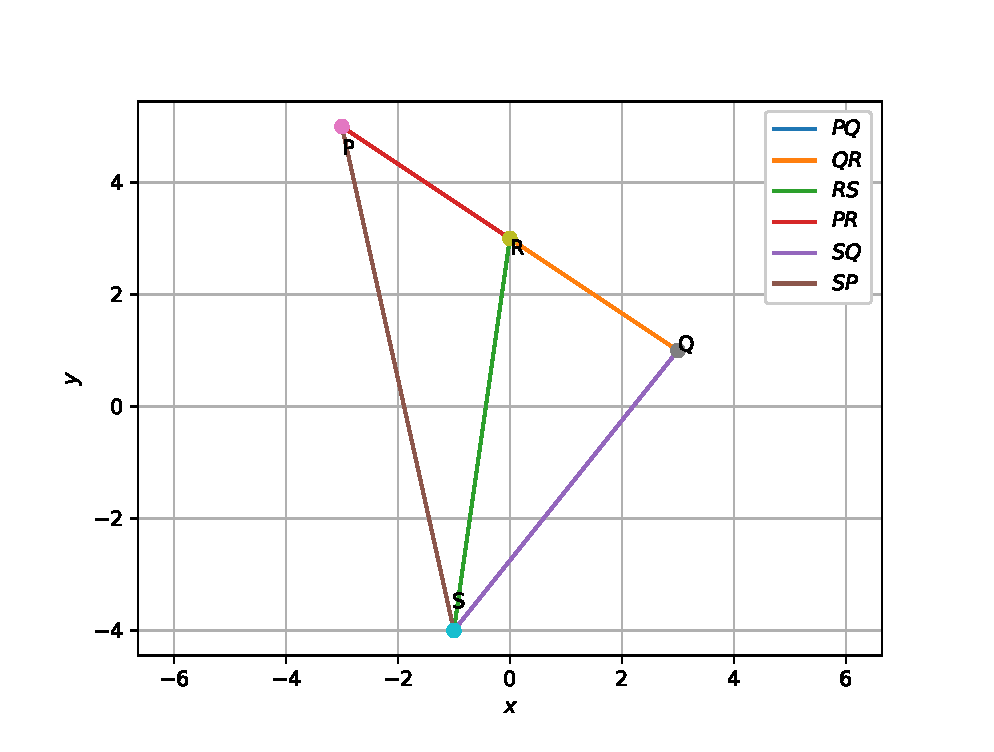
\includegraphics[width=\columnwidth]{./figures/quad2.eps}
	\caption{quadrilateral2 }
	\label{fig:quadrilateral2}
\end{figure}
\begin{lstlisting}
codes/quad1.py
\end{lstlisting}
\end{enumerate}